\documentclass[10pt,a4paper, enlgish, spanish]{article}

\usepackage{color}     % para snipets de codigo coloreados
\usepackage{amsmath}
\usepackage{amsfonts}
\usepackage[utf8]{inputenc}
\usepackage[T1]{fontenc}
\usepackage{geometry}
 \geometry{
    a4paper,
    total={210mm,297mm},
    left=5mm,
    right=5mm,
    top=15mm,
    bottom=15mm
 }

\usepackage{dependencies/caratula,dependencies/aed2-symb,dependencies/aed2-itef,dependencies/aed2-tad, dependencies/aed2-helper}
\usepackage[spanish]{babel}
\usepackage{fancyhdr}
\usepackage{algorithm2e}
\usepackage{algpseudocode}
\usepackage{listings}
\usepackage{xcolor}
\usepackage{pdfpages} 
\usepackage{fancybox}  % para el sbox de los snipets de codigo
\usepackage{graphicx}

\usepackage{caption}
\usepackage{subcaption}
\usepackage{float}
\usepackage{lastpage}
\usepackage{afterpage}


% definiciones

\newtheorem{theorem}{Teorema}[section]
\newtheorem{lemma}[theorem]{Lema}
\newtheorem{proposition}[theorem]{Proposici\'on}
\newtheorem{corollary}[theorem]{Corolario}

\newcommand{\Var}{\textbf{var }}
\newcommand{\True}{\textbf{true }}
\newcommand{\False}{\textbf{false }}
\newcommand{\Break}{\textbf{break }}

\newenvironment{proof}[1][Demostraci\'on]{\begin{trivlist}
\item[\hskip \labelsep {\bfseries #1}]}{\end{trivlist}}
\newenvironment{definition}[1][Definici\'on]{\begin{trivlist}
\item[\hskip \labelsep {\bfseries #1}]}{\end{trivlist}}
\newenvironment{example}[1][Ejemplo]{\begin{trivlist}
\item[\hskip \labelsep {\bfseries #1}]}{\end{trivlist}}
\newenvironment{remark}[1][Observaci\'on]{\begin{trivlist}
\item[\hskip \labelsep {\bfseries #1}]}{\end{trivlist}}

\definecolor{litegrey}{gray}{0.94}

\newenvironment{codesnippet}{%
	\begin{Sbox}\begin{minipage}{\textwidth}\sffamily\small}%
	{\end{minipage}\end{Sbox}%
		\begin{center}%
		\vspace{-0.4cm}\colorbox{litegrey}{\TheSbox}\end{center}\vspace{0.3cm}}

\lstset{frame=tb,
	  language=Java,
	  aboveskip=3mm,
	  belowskip=3mm,
	  showstringspaces=false,
	  columns=flexible,
	  basicstyle={\scriptsize\ttfamily},
	  numberstyle=\tiny\color{gray},
	  keywordstyle=\color{blue},
	  commentstyle=\color{green},
	  stringstyle=\color{red},
	  breaklines=true,
	  breakatwhitespace=true,
	  tabsize=3,
	  numbers=left,
	  numbersep=15pt,
	  numberfirstline = false
	}


\begin{document}

% **************************************************************************
%
%  Package 'caratula', version 0.2 (para componer caratulas de TPs del DC).
%
%  En caso de dudas, problemas o sugerencias sobre este package escribir a
%  Nico Rosner (nrosner arroba dc.uba.ar).
%
% **************************************************************************



% ----- Informacion sobre el package para el sistema -----------------------

\NeedsTeXFormat{LaTeX2e}
\ProvidesPackage{caratula}[2003/4/13 v0.1 Para componer caratulas de TPs del DC]


% ----- Imprimir un mensajito al procesar un .tex que use este package -----

\typeout{Cargando package 'caratula' v0.2 (21/4/2003)}


% ----- Algunas variables --------------------------------------------------

\let\Materia\relax
\let\Submateria\relax
\let\Titulo\relax
\let\Subtitulo\relax
\let\Grupo\relax


% ----- Comandos para que el usuario defina las variables ------------------

\def\materia#1{\def\Materia{#1}}
\def\submateria#1{\def\Submateria{#1}}
\def\titulo#1{\def\Titulo{#1}}
\def\subtitulo#1{\def\Subtitulo{#1}}
\def\grupo#1{\def\Grupo{#1}}


% ----- Token list para los integrantes ------------------------------------

\newtoks\intlist\intlist={}


% ----- Comando para que el usuario agregue integrantes

\def\integrante#1#2#3{\intlist=\expandafter{\the\intlist
    \rule{0pt}{1.2em}#1&#2&\tt #3\\[0.2em]}}


% ----- Macro para generar la tabla de integrantes -------------------------

\def\tablaints{%
    \begin{tabular}{|l@{\hspace{4ex}}c@{\hspace{4ex}}l|}
        \hline
        \rule{0pt}{1.2em}Integrante & LU & Correo electr\'onico\\[0.2em]
        \hline
        \the\intlist
        \hline
    \end{tabular}}

% ----- Macro para generar la parte reservada para la c�tedra -------------------------

\def\tablacatedra{%
    \\
    \textbf{Reservado para la cátedra}\par\bigskip
    \begin{tabular}{|c|c|c|}
        \hline
        \rule{0pt}{1.2em}Instancia & Docente & Nota\\[0.2em]
        \hline
        \rule{0pt}{1.2em}Primera entrega & \phantom{mmmmmmmmmmmmmmmmmm} & \phantom{mmmmmm} \\
        \hline
        \rule{0pt}{1.2em}Segunda entrega & & \\
        \hline
    \end{tabular}}

% ----- Codigo para manejo de errores --------------------------------------

\def\se{\let\ifsetuperror\iftrue}
\def\ifsetuperror{%
    \let\ifsetuperror\iffalse
    \ifx\Materia\relax\se\errhelp={Te olvidaste de proveer una \materia{}.}\fi
    \ifx\Titulo\relax\se\errhelp={Te olvidaste de proveer un \titulo{}.}\fi
    \edef\mlist{\the\intlist}\ifx\mlist\empty\se%
    \errhelp={Tenes que proveer al menos un \integrante{nombre}{lu}{email}.}\fi
    \expandafter\ifsetuperror}


% ----- Reemplazamos el comando \maketitle de LaTeX con el nuestro ---------

\def\maketitle{%
    \ifsetuperror\errmessage{Faltan datos de la caratula! Ingresar 'h' para mas informacion.}\fi
    \thispagestyle{empty}
    \begin{center}
    \vspace*{\stretch{2}}
    {\LARGE\textbf{\Materia}}\\[1em]
    \ifx\Submateria\relax\else{\Large \Submateria}\\[0.5em]\fi
    \par\vspace{\stretch{1}}
    {\large Departamento de Computaci\'on}\\[0.5em]
    {\large Facultad de Ciencias Exactas y Naturales}\\[0.5em]
    {\large Universidad de Buenos Aires}
    \par\vspace{\stretch{3}}
    {\Large \textbf{\Titulo}}\\[0.8em]
    {\Large \Subtitulo}
    \par\vspace{\stretch{3}}
    \ifx\Grupo\relax\else\textbf{\Grupo}\par\bigskip\fi
    \tablaints
    \vspace*{\stretch{3}}
    \medskip
    \\
    En el presente trabajo recrearemos una imagen 3D utilizando el modelo de fotometría stéreo para el cálculo de la profunidad de la misma a partir de diversas fuentes lumínicas. Compararemos los métodos de Eliminación Gaussiana y factorización de Cholesky utilizadas para resolver los sistemas de ecuaciones lineales involucrados en el cálculo de la profunidad en función de la carga computación y de la calidad de los resutlados obetnidos.
    \\
    \vspace*{\stretch{3}}
    {\bf Palabras claves:} Eliminación Gaussiana, Cholesky, Fotometría Estéreo.
    \vspace*{\stretch{3}}
    \medskip
    \tablacatedra
    \end{center}
    \vspace*{\stretch{3}}
    \newpage
    }
\newpage

\tableofcontents
\newpage

\section{Introducción}

En este trabajo práctico abordaremos la temática de la reconstrucción de objetos tridimensionales utilizando de tales objetos fotografías bidimensionales. Para ello, emplearemos técnicas de fotometría estéreo, que derivarán en la aplicación de métodos numéricos de resolución de sistemas de ecuaciones lineales.
\\
Contamos con una colección de fotografías correspondientes a distintos objetos. Por cada objeto, contamos con doce fotografías, tomadas cada una desde la misma posición de cámara, pero ubicando la fuente de luz en distintos puntos del espacio. Las doce ubicaciones de la fuente lumínica son las mismas para las fotografías de todos los objetos.

Tal como se detalla en el enunciado del trabajo, es necesario descubrir la posición de las fuentes de iluminación, para lo que se pasa por una etapa de Calibración. 
\\

Una vez realizada la calibración, se puede pasar a esrtimar la forma tridimensional de alguno de los objetos. Para ello, deben escogerse tres fotografías del mismo objeto, desde tres focos de iluminación distintos, ya conocidos.
\\

Hecho esto, se debe calcular, para cada píxel de la imagen el vector normal a la superficie del objeto, formando el sistema de ecuaciones (5) del enunciado para cada píxel.
\\

A continuación, se arma el sistema de ecuaciones general, detallado en las ecuaciones (11) y (12) del enunciado, y se forma con ellos la matriz $M$, a partir de la cual se forma la matriz $A$ $=$ $M$ $^{t}$ $M$. 
\\

La resolución de los sistemas de ecuaciones se hace con los métodos de Eliminación Gaussiana Clásica y Factorización de Cholesky \cite{burden}.
\\
La utilización de estos métodos de resolución exigen condiciones de la matriz en cuestión. A continuación, detallamos el cumplimiento de la matriz $A$ de tales condiciones.
\\

\textbf{Demostración de que se puede aplicar Eliminación Gaussiana Clásica (sin pivoteo) y Factorización de CHolesky sobre la matriz $A$ $=$ $M$ $^{t}$ $M$.}
\\

1) \textit{M es inversible}: Se puede ver observando las ecuaciones que la constituyen y notando que, para cualesquiera dos filas de M (cualesquiera dos ecuaciones), va a haber al menos una incógnita en la que una tenga coeficiente nula y la otra no; es decir, para cualesquiera dos filas de M, va a haber al menos una columna en la que una tenga valor 0 y la otra no. \\
Además, los elementos de la diagonal representan valores de una dimensión de las normales a la superficie. En el contexto del problema, no tiene sentido que este valor sea 0.\\
Es decir, no habrá columnas nulas en la matriz M. Esto hace que las filas de M sean linealmente independientes, y es hace a M inversible.
\\

2) Al ser M inversible, lo son también $M$ $^{t}$ y A (por ser producto de inversibles)
\\

3)\textit{A es simétrica: } (trivial transponiendo($M$ $^{t}$ $M$))\\

\textit{A es definida positiva:} sup $x$ $\in$ $\mathbb{R}$ $^{n}$, $x \ne 0$ 
arbitrario. \\

x$^{t}$ $A$ $x$  = $x$ $^{t}$ $M$ $^{t}$ $M$ $ x$ $=$ ($Mx$)$^{t}$ 
 $(M*x)$ = $\|$ $Mx$ $\|$ $>$ $0$ por ser $x$ $\neq$ $0$ y $M$ 
inversible. \\

Por lo tanto, A es SDP, y por ende, puede aplicársele la factorización de CHolesky.
\\

4)
A es simétrica definida positiva $\implies$ (por ej 7/c de la práctica 3) Todas las submatrices principales de A son definidas positivas $\implies$ (por ej 7/b de la práctica 3) Todas las submatrices principales de A son no singulares $\implies$ (por ej 7 de la práctica 2)  A admite factorización LU sin pivoteo (y además es única) - que es equivalente a decir que sobre A se puede aplicar Eliminación Gaussiana Clásica
\\

\newpage

\section{Desarrollo}

En esta secci\'on expondremos el camino recorrido durante la construcci\'on del trabajo, las dificultades encontradas y la forma final del mismo.

\subsection{Implementaci\'on de algoritmos y estructuras de datos accesorias}

El primer problema a resolver fue la generaci\'on del programa que resuelva las exigencias del trabajo pr\'actico: la calibraci\'on, el c\'alculo de normales y la codificaci\'on concreta de los algoritmos te\'oricos \emph{Eliminaci\'on Gaussiana Cl\'asica} (sin pivoteo) y \emph{Factorizaci\'on de Cholesky}. 

\subsubsection {Etapa de Calibraci\'on}
Para la calibraci\'on de las fuentes lum\'inicas utilizamos las fotograf\'ias de las esferas. De esta figura conocemos su geometr\'ia, permitiendonos as\'i hallar la direcci\'on de iluminaci\'on. 

El primer paso de la calibraci\'on es calcular el radio y centro de la esfera. Utilizamos la m\'ascara provista para que solo hayan puntos negros y blancos. En esta medimos la mayor y menor componente x e y de los puntos blancos. Luego la componente x e y del centro es el promedio del m\'aximo y del m\'inimo, y el di\'ametro es la diferencia.

Una vez obtenidos los parametros de la esfera, procedemos a econtrar el punto m\'as brillante. Esta no es una tarea sencilla ya que pueden haber varios puntos brillantes (la foto puede estar saturada, o la resoluci\'on de los pixeles no permiten diferenciar) o bien la superficie de la esfera puede hacer brillar m\'as un punto alejado de la zona más brillante. Por esta raz\'on, en vez de tomar el punto m\'as brillante directamente, tomamos el promedio ponderado de todos los puntos con el brillo del p\'ixel como peso. Asi los puntos brillantes aislados influyen menos en la elecci\'on.

Con el punto m\'as brillante y con los par\'ametros de la esfera ya es posible calcular la normal. El punto es la proyecci\'on al plano de un punto de la esfera. La ecuaci\'on impl\'icita de la esfera es $F(x,y,z) = (x-x_0)^2+(y-y_0)^2+(z-z_0)^2 = r^2$ donde $(x_0,y_0,z_0)$ y $r$ son el centro y el radio de la esfera. En nuestro fijamos $z_0 = 0$(cualquier $z_0$ nos dar\'a el mismo resultado). Despejando $z = \sqrt{r^2 - (x-x0)^2 - (y-y0)^2}$. De esta forma obtenemos el punto de la esfera.

Por Teorema de la Funci\'on Impl\'icita, la normal a la superficie en el punto $(x,y,z)$ esta dado por el gradiente de $F$. En la esfera $\nabla F(x,y,z) = 2(x-x_0,y-y_0,z)$, o sea al calcular el punto m\'as brillante en la esfera ya obtuvimos la direcci\'on del haz.

\subsubsection {C\'alculo de normales por p\'ixel}

Contando con el dato de la ubicación de cada una de las doce fuentes lumínicas, se deben escoger tres fotografías de un mismo objeto, iluminadas desde tres fuentes distintas. Con esta información, se puede calcular la normal a la superficie del objeto para cada punto del objeto (representado por un píxel en cada una de las tres imágenes).

El sistema de ecuaciones formulado es el sistema (5) del enunciado del trabajo. 
Dado que las ecuaciones son las mismas para todos los píxeles de la imagen, excepto por el término independiente, la matriz que se forma puede ser factorizada con el método LU (ó PLU), de modo de ahorrar cálculos que se repiten en cada píxel.

\subsubsection{Construcci\'on del sistema de ecuaciones principal}

Una vez escogidas las im\'agenes a utilizar y calculadas las normales de cada p\'ixel, debe procederse a estimar las profundidades de cada p\'ixel. Para ello, se formula el sistema de ecuaciones presentado en la Introducci\'on, formando la matriz $M$.

La matriz M consta de una columna y dos filas (correspondientes a dos ecuaciones) por cada p\'ixel de la imagen tomada. Los p\'ixeles de una fila los ordenamos por filas de la imagen. Es decir, primero se ubican los p\'ixeles de la primer fila de la imagen, a continuaci\'on los p\'ixeles de la segunda fila de la im\'agen, etc\'etera.

Esta conformaci\'on provoca que, para los p\'ixeles de la \'ultima fila (la de m\'as abajo) de la imagen, algunos de los elementos de las ecuaciones no se encuentren definidos. Decidimos, para estas ecuaciones s\'olo incluir los elementos definidos.
Elegida esta disposici\'on de elementos y exclusi\'on de elementos no definidos, la matriz $M$ resulta una matriz esparsa banda, de dimensiones $2NxN$, donde $N$ es la cantidad de p\'ixeles de la imagen.
Por tanto, la matriz $A$ (igual a $M^t * M$) resulta de dimensiones $N X N$, tambien banda y marcadamente esparsa.

\subsubsection {Resoluci\'on del sistema de ecuaciones principal: 
Implementaciones preliminares descartadas}

El problema que se presenta, decididos los elementos que deben formar la matriz $A$, es implementar las estructuras de datos para alojarla y los algoritmos para resolver el sistema de ecuaciones.

Durante el transcurso de la resoluci\'on del trabajo, se usaron, descartaron y perfeccionaron versiones del programa, hasta llegar a su forma final.

La primer aproximaci\'on utilizada fue la m\'as natural de todas: implementar la matriz como un arreglo de arreglos de números (en lenguaje C++, esto se puede hacer con la clase vector<vector<double\textgreater\textgreater), y los algoritmos EG y CH tal como se presentan en la bibliografía citada. Esto es, recorriendo cada elemento de la matriz que corresponda al método. 
Sin embargo, dado que las imágenes provistas por la cátedra tienen aproximadamente 170.000 píxeles, una matriz $A$ consta de aproximadamente 30.000.000.000 elementos. Al intentar generar una instancia de vector<vector<double\textgreater\textgreater de 30.000.000.000 elementos en total, se saturaron las capacidades de memoria de las computadoras en que se intentó hacerlo.
Por lo tanto, esta aproximación fue descartada.

El segundo intento fue cambiar la estructura de datos de soporte de la matriz, de vector<vector<double\textgreater\textgreater, que aloja todos los valores de la matriz, a una que sólo aloje los valores no nulos, teniendo en cuenta que se trabajará con matrices esparsas. Esa estructura de datos elegida fue map<pair<int,int\textgreater ,double \textgreater, un diccionario cuyas claves representan una posición de la matriz <fila,columna\textgreater, y el valor correspondiente es el elemento de la matriz referenciado, y sólo se almacenan los valores no nulos de la matriz.
Con esta nueva estructura de datos, se logró cargar las matrices en memoria. No obstante, los algoritmos implementados seguían recorriendo todas las posiciones de la matriz, constituyendo un algoritmo de complejidad temporal cuadrático. La ejecución de estos algoritmos se proyectaba en alrededor de 40 horas en promedio.

Una tercer mejoría consistió en tratar de aprovechar la característica de ser banda de las matrices a trabajar. Se intentó hacer esto anexando a la matriz una estructura de datos en la que, para cada fila, se guardara la máxima y mínima columna de valor no nulo, y análogamente para cada columna, la máxima y mínima columna de valor no nulo. Tal estructura de datos fue vector<pair<int,int\textgreater\textgreater, que guardaba en cada posición (correspondiente a cada fila o columna), la máxima fila o columna no nula. Esto permitió alterar los algoritmos EG y CH, de modo que sólo recorran la banda de valores no nulos para cada fila o columna. De este modo, la el tiempo promedio de ejecución de los algoritmos pasó a ser de aproximadamente de 4 horas.

No obstante, se pudo realizar una mejora adicional.

\subsubsection{Resoluci\'on del sistema de ecuaciones principal: 
Implementaci\'on definitiva}

La implementación final de la resolución del sistema de ecuaciones utiliza como estructura de datos accesoria un vector que, para cada fila, indica cada una de las columnas en las que hay un valor no nulo. Análogamente, otro vector para cada columna indica cada una de las filas en las que hay un valor no nulo. Estas estructuras se implementan con dos instancias de la clase vector<set<int\textgreater\textgreater. Al ser set un conjunto ordenado, esto permite que los algoritmos EG y CH recorrer, para cada fila o columna, según corresponda, sólo las posiciones en las que hay valores no nulos.
Aprovechando el hecho de que la matriz es esparsa, y hay muy pocos elementos no nulos, esto vueve a los algoritmos lineales en cuanto a su complejidad temporal.




\newpage

\section{Resultados y discusión}

\section{Resultados y discusión}

\subsection{Análisis Cuantitativo}
\subsubsection{Tiempo de Cómputo}
\textbf{Objetivo}:
El objetivo de este experimento consiste en determinar el tiempo de cómputo de ambos métodos y compararlos en función del tamaño de la entrada.
\\
\textbf{Hipótesis:}

\textbf{Resultados y discusión:}


\subsection{Análisis Cualitativo}
\subsubsection{Comparación de direcciones de iluminación}
\textbf{Objetivo}:
El objetivo de este experimento es 
\\
\textbf{Hipótesis:}

\textbf{Resultados y discusión:}


\subsubsection{Efecto de la calibración en el resto de las etapas}
\textbf{Objetivo}:
El objetivo de este experimento es 
\\
\textbf{Hipótesis:}

\textbf{Resultados y discusión:}


\subsubsection{Impacto de las direcciones de iluminación en el cálculo de las normales}
\textbf{Objetivo}:
El objetivo de este experimento es 

\textbf{Hipótesis:}

\textbf{Resultados y discusión:}
\newpage

\section{Conclusión}


\newpage

\section{Apéndice} \label{cap:apendice}

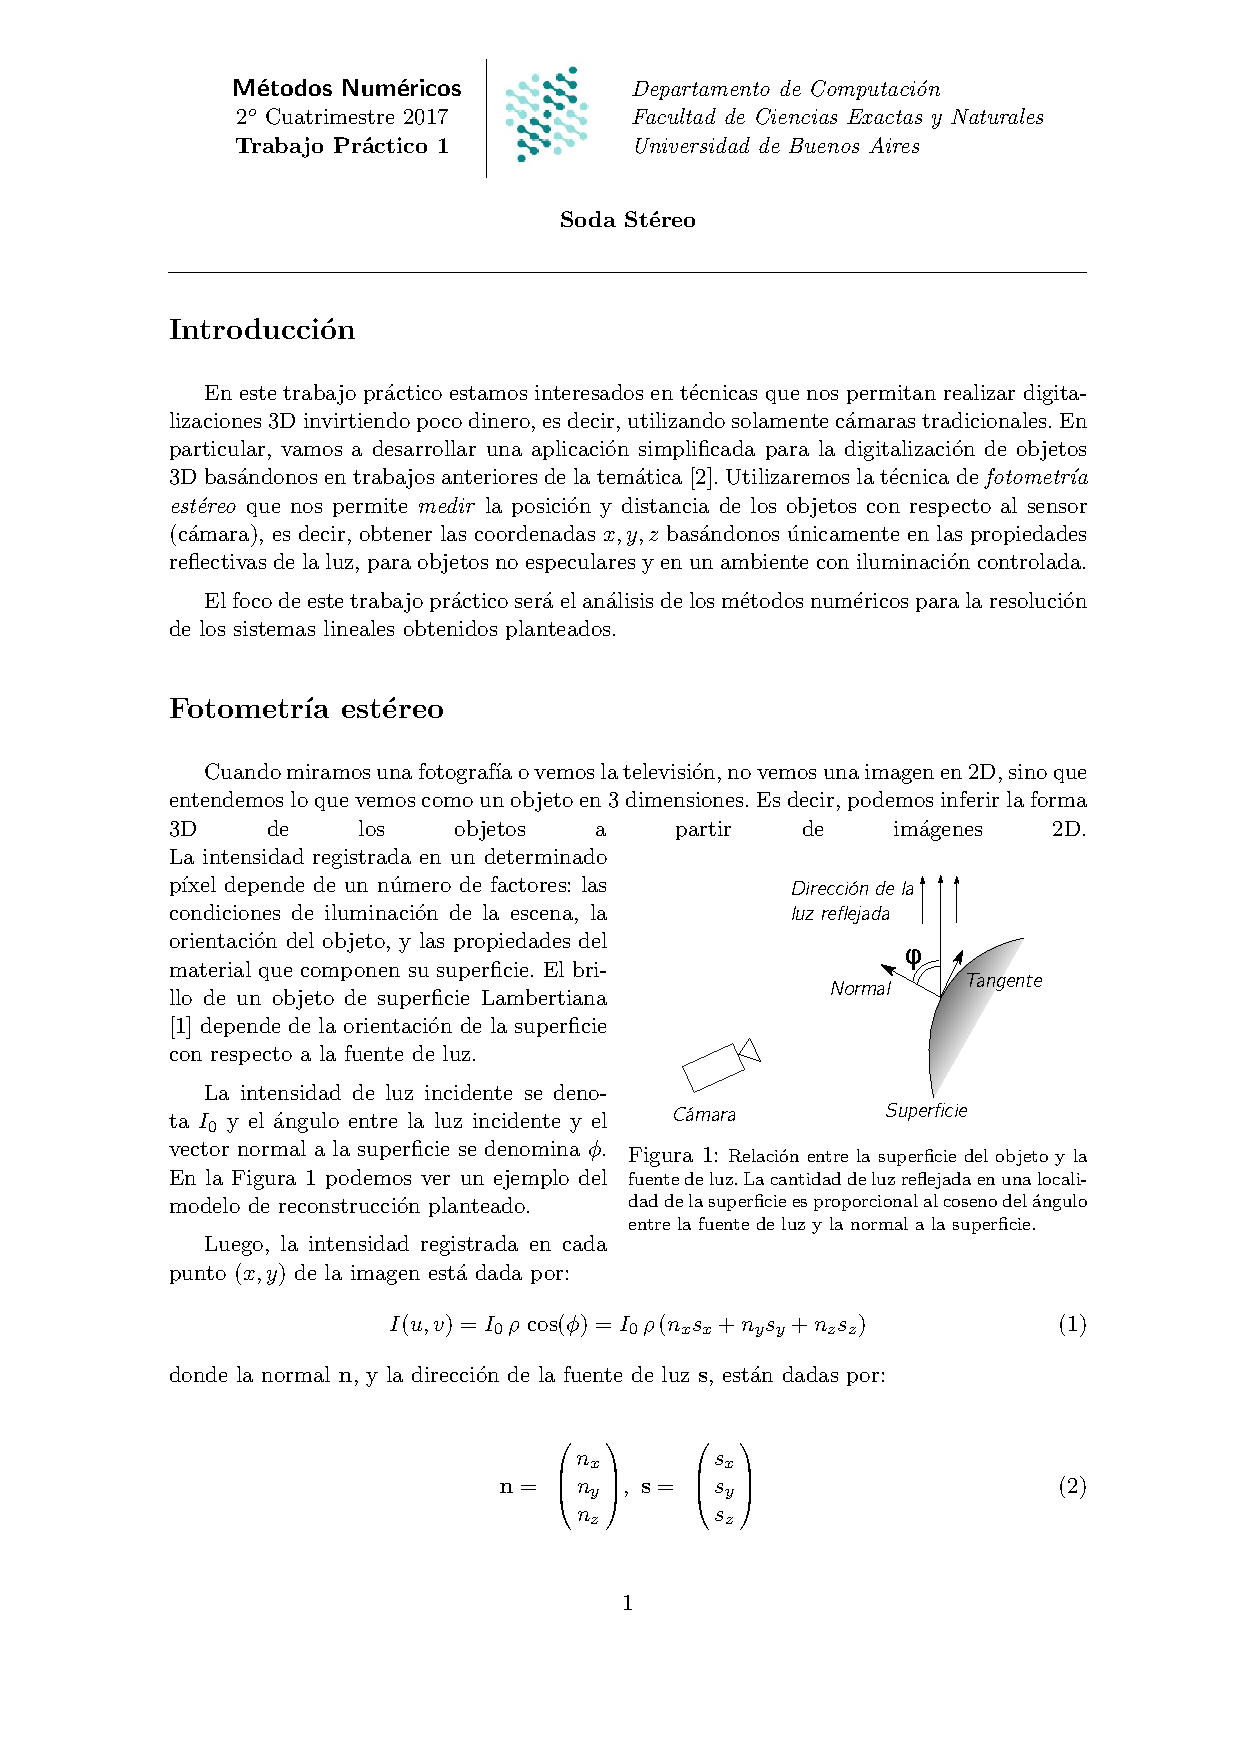
\includepdf[pages=-]{../enunciado/tp1.pdf}

\newpage

\section{Referencias}

 
\begin{thebibliography}{9}


\end{thebibliography}



%\input{others/comentarios}

\end{document}
